
%% bare_conf.tex
%% V1.3
%% 2007/01/11
%% by Michael Shell
%% See:
%% http://www.michaelshell.org/
%% for current contact information.
%%
%% This is a skeleton file demonstrating the use of IEEEtran.cls
%% (requires IEEEtran.cls version 1.7 or later) with an IEEE conference paper.
%%
%% Support sites:
%% http://www.michaelshell.org/tex/ieeetran/
%% http://www.ctan.org/tex-archive/macros/latex/contrib/IEEEtran/
%% and
%% http://www.ieee.org/

%%*************************************************************************
%% Legal Notice:
%% This code is offered as-is without any warranty either expressed or
%% implied; without even the implied warranty of MERCHANTABILITY or
%% FITNESS FOR A PARTICULAR PURPOSE! 
%% User assumes all risk.
%% In no event shall IEEE or any contributor to this code be liable for
%% any damages or losses, including, but not limited to, incidental,
%% consequential, or any other damages, resulting from the use or misuse
%% of any information contained here.
%%
%% All comments are the opinions of their respective authors and are not
%% necessarily endorsed by the IEEE.
%%
%% This work is distributed under the LaTeX Project Public License (LPPL)
%% ( http://www.latex-project.org/ ) version 1.3, and may be freely used,
%% distributed and modified. A copy of the LPPL, version 1.3, is included
%% in the base LaTeX documentation of all distributions of LaTeX released
%% 2003/12/01 or later.
%% Retain all contribution notices and credits.
%% ** Modified files should be clearly indicated as such, including  **
%% ** renaming them and changing author support contact information. **
%%
%% File list of work: IEEEtran.cls, IEEEtran_HOWTO.pdf, bare_adv.tex,
%%                    bare_conf.tex, bare_jrnl.tex, bare_jrnl_compsoc.tex
%%*************************************************************************

% *** Authors should verify (and, if needed, correct) their LaTeX system  ***
% *** with the testflow diagnostic prior to trusting their LaTeX platform ***
% *** with production work. IEEE's font choices can trigger bugs that do  ***
% *** not appear when using other class files.                            ***
% The testflow support page is at:
% http://www.michaelshell.org/tex/testflow/



% Note that the a4paper option is mainly intended so that authors in
% countries using A4 can easily print to A4 and see how their papers will
% look in print - the typesetting of the document will not typically be
% affected with changes in paper size (but the bottom and side margins will).
% Use the testflow package mentioned above to verify correct handling of
% both paper sizes by the user's LaTeX system.
%
% Also note that the "draftcls" or "draftclsnofoot", not "draft", option
% should be used if it is desired that the figures are to be displayed in
% draft mode.
%
\documentclass[conference]{IEEEtran}
% Add the compsoc option for Computer Society conferences.
%
% If IEEEtran.cls has not been installed into the LaTeX system files,
% manually specify the path to it like:
% \documentclass[conference]{../sty/IEEEtran}





% Some very useful LaTeX packages include:
% (uncomment the ones you want to load)


% *** MISC UTILITY PACKAGES ***
%
%\usepackage{ifpdf}
% Heiko Oberdiek's ifpdf.sty is very useful if you need conditional
% compilation based on whether the output is pdf or dvi.
% usage:
% \ifpdf
%   % pdf code
% \else
%   % dvi code
% \fi
% The latest version of ifpdf.sty can be obtained from:
% http://www.ctan.org/tex-archive/macros/latex/contrib/oberdiek/
% Also, note that IEEEtran.cls V1.7 and later provides a builtin
% \ifCLASSINFOpdf conditional that works the same way.
% When switching from latex to pdflatex and vice-versa, the compiler may
% have to be run twice to clear warning/error messages.






% *** CITATION PACKAGES ***
%
\usepackage{cite}
% cite.sty was written by Donald Arseneau
% V1.6 and later of IEEEtran pre-defines the format of the cite.sty package
% \cite{} output to follow that of IEEE. Loading the cite package will
% result in citation numbers being automatically sorted and properly
% "compressed/ranged". e.g., [1], [9], [2], [7], [5], [6] without using
% cite.sty will become [1], [2], [5]--[7], [9] using cite.sty. cite.sty's
% \cite will automatically add leading space, if needed. Use cite.sty's
% noadjust option (cite.sty V3.8 and later) if you want to turn this off.
% cite.sty is already installed on most LaTeX systems. Be sure and use
% version 4.0 (2003-05-27) and later if using hyperref.sty. cite.sty does
% not currently provide for hyperlinked citations.
% The latest version can be obtained at:
% http://www.ctan.org/tex-archive/macros/latex/contrib/cite/
% The documentation is contained in the cite.sty file itself.






% *** GRAPHICS RELATED PACKAGES ***
%
\ifCLASSINFOpdf
  \usepackage[pdftex]{graphicx}
  % declare the path(s) where your graphic files are
  % \graphicspath{{../pdf/}{../jpeg/}}
  % and their extensions so you won't have to specify these with
  % every instance of \includegraphics
  \DeclareGraphicsExtensions{.pdf,.jpeg,.png}
\else
  % or other class option (dvipsone, dvipdf, if not using dvips). graphicx
  % will default to the driver specified in the system graphics.cfg if no
  % driver is specified.
  \usepackage[dvips]{graphicx}
  % declare the path(s) where your graphic files are
  % \graphicspath{{../eps/}}
  % and their extensions so you won't have to specify these with
  % every instance of \includegraphics
  \DeclareGraphicsExtensions{.eps}
\fi
% graphicx was written by David Carlisle and Sebastian Rahtz. It is
% required if you want graphics, photos, etc. graphicx.sty is already
% installed on most LaTeX systems. The latest version and documentation can
% be obtained at: 
% http://www.ctan.org/tex-archive/macros/latex/required/graphics/
% Another good source of documentation is "Using Imported Graphics in
% LaTeX2e" by Keith Reckdahl which can be found as epslatex.ps or
% epslatex.pdf at: http://www.ctan.org/tex-archive/info/
%
% latex, and pdflatex in dvi mode, support graphics in encapsulated
% postscript (.eps) format. pdflatex in pdf mode supports graphics
% in .pdf, .jpeg, .png and .mps (metapost) formats. Users should ensure
% that all non-photo figures use a vector format (.eps, .pdf, .mps) and
% not a bitmapped formats (.jpeg, .png). IEEE frowns on bitmapped formats
% which can result in "jaggedy"/blurry rendering of lines and letters as
% well as large increases in file sizes.
%
% You can find documentation about the pdfTeX application at:
% http://www.tug.org/applications/pdftex





% *** MATH PACKAGES ***
%
\usepackage[cmex10]{amsmath}
% A popular package from the American Mathematical Society that provides
% many useful and powerful commands for dealing with mathematics. If using
% it, be sure to load this package with the cmex10 option to ensure that
% only type 1 fonts will utilized at all point sizes. Without this option,
% it is possible that some math symbols, particularly those within
% footnotes, will be rendered in bitmap form which will result in a
% document that can not be IEEE Xplore compliant!
%
% Also, note that the amsmath package sets \interdisplaylinepenalty to 10000
% thus preventing page breaks from occurring within multiline equations. Use:
%\interdisplaylinepenalty=2500
% after loading amsmath to restore such page breaks as IEEEtran.cls normally
% does. amsmath.sty is already installed on most LaTeX systems. The latest
% version and documentation can be obtained at:
% http://www.ctan.org/tex-archive/macros/latex/required/amslatex/math/





% *** SPECIALIZED LIST PACKAGES ***
%
%\usepackage{algorithmic}
% algorithmic.sty was written by Peter Williams and Rogerio Brito.
% This package provides an algorithmic environment fo describing algorithms.
% You can use the algorithmic environment in-text or within a figure
% environment to provide for a floating algorithm. Do NOT use the algorithm
% floating environment provided by algorithm.sty (by the same authors) or
% algorithm2e.sty (by Christophe Fiorio) as IEEE does not use dedicated
% algorithm float types and packages that provide these will not provide
% correct IEEE style captions. The latest version and documentation of
% algorithmic.sty can be obtained at:
% http://www.ctan.org/tex-archive/macros/latex/contrib/algorithms/
% There is also a support site at:
% http://algorithms.berlios.de/index.html
% Also of interest may be the (relatively newer and more customizable)
% algorithmicx.sty package by Szasz Janos:
% http://www.ctan.org/tex-archive/macros/latex/contrib/algorithmicx/




% *** ALIGNMENT PACKAGES ***
%
%\usepackage{array}
% Frank Mittelbach's and David Carlisle's array.sty patches and improves
% the standard LaTeX2e array and tabular environments to provide better
% appearance and additional user controls. As the default LaTeX2e table
% generation code is lacking to the point of almost being broken with
% respect to the quality of the end results, all users are strongly
% advised to use an enhanced (at the very least that provided by array.sty)
% set of table tools. array.sty is already installed on most systems. The
% latest version and documentation can be obtained at:
% http://www.ctan.org/tex-archive/macros/latex/required/tools/


%\usepackage{mdwmath}
%\usepackage{mdwtab}
% Also highly recommended is Mark Wooding's extremely powerful MDW tools,
% especially mdwmath.sty and mdwtab.sty which are used to format equations
% and tables, respectively. The MDWtools set is already installed on most
% LaTeX systems. The lastest version and documentation is available at:
% http://www.ctan.org/tex-archive/macros/latex/contrib/mdwtools/


% IEEEtran contains the IEEEeqnarray family of commands that can be used to
% generate multiline equations as well as matrices, tables, etc., of high
% quality.


%\usepackage{eqparbox}
% Also of notable interest is Scott Pakin's eqparbox package for creating
% (automatically sized) equal width boxes - aka "natural width parboxes".
% Available at:
% http://www.ctan.org/tex-archive/macros/latex/contrib/eqparbox/





% *** SUBFIGURE PACKAGES ***
%\usepackage[tight,footnotesize]{subfigure}
% subfigure.sty was written by Steven Douglas Cochran. This package makes it
% easy to put subfigures in your figures. e.g., "Figure 1a and 1b". For IEEE
% work, it is a good idea to load it with the tight package option to reduce
% the amount of white space around the subfigures. subfigure.sty is already
% installed on most LaTeX systems. The latest version and documentation can
% be obtained at:
% http://www.ctan.org/tex-archive/obsolete/macros/latex/contrib/subfigure/
% subfigure.sty has been superceeded by subfig.sty.



%\usepackage[caption=false]{caption}
%\usepackage[font=footnotesize]{subfig}
% subfig.sty, also written by Steven Douglas Cochran, is the modern
% replacement for subfigure.sty. However, subfig.sty requires and
% automatically loads Axel Sommerfeldt's caption.sty which will override
% IEEEtran.cls handling of captions and this will result in nonIEEE style
% figure/table captions. To prevent this problem, be sure and preload
% caption.sty with its "caption=false" package option. This is will preserve
% IEEEtran.cls handing of captions. Version 1.3 (2005/06/28) and later 
% (recommended due to many improvements over 1.2) of subfig.sty supports
% the caption=false option directly:
%\usepackage[caption=false,font=footnotesize]{subfig}
%
% The latest version and documentation can be obtained at:
% http://www.ctan.org/tex-archive/macros/latex/contrib/subfig/
% The latest version and documentation of caption.sty can be obtained at:
% http://www.ctan.org/tex-archive/macros/latex/contrib/caption/




% *** FLOAT PACKAGES ***
%
\usepackage{fixltx2e}
% fixltx2e, the successor to the earlier fix2col.sty, was written by
% Frank Mittelbach and David Carlisle. This package corrects a few problems
% in the LaTeX2e kernel, the most notable of which is that in current
% LaTeX2e releases, the ordering of single and double column floats is not
% guaranteed to be preserved. Thus, an unpatched LaTeX2e can allow a
% single column figure to be placed prior to an earlier double column
% figure. The latest version and documentation can be found at:
% http://www.ctan.org/tex-archive/macros/latex/base/



%\usepackage{stfloats}
% stfloats.sty was written by Sigitas Tolusis. This package gives LaTeX2e
% the ability to do double column floats at the bottom of the page as well
% as the top. (e.g., "\begin{figure*}[!b]" is not normally possible in
% LaTeX2e). It also provides a command:
%\fnbelowfloat
% to enable the placement of footnotes below bottom floats (the standard
% LaTeX2e kernel puts them above bottom floats). This is an invasive package
% which rewrites many portions of the LaTeX2e float routines. It may not work
% with other packages that modify the LaTeX2e float routines. The latest
% version and documentation can be obtained at:
% http://www.ctan.org/tex-archive/macros/latex/contrib/sttools/
% Documentation is contained in the stfloats.sty comments as well as in the
% presfull.pdf file. Do not use the stfloats baselinefloat ability as IEEE
% does not allow \baselineskip to stretch. Authors submitting work to the
% IEEE should note that IEEE rarely uses double column equations and
% that authors should try to avoid such use. Do not be tempted to use the
% cuted.sty or midfloat.sty packages (also by Sigitas Tolusis) as IEEE does
% not format its papers in such ways.





% *** PDF, URL AND HYPERLINK PACKAGES ***
%
\usepackage{url}
% url.sty was written by Donald Arseneau. It provides better support for
% handling and breaking URLs. url.sty is already installed on most LaTeX
% systems. The latest version can be obtained at:
% http://www.ctan.org/tex-archive/macros/latex/contrib/misc/
% Read the url.sty source comments for usage information. Basically,
% \url{my_url_here}.





% *** Do not adjust lengths that control margins, column widths, etc. ***
% *** Do not use packages that alter fonts (such as pslatex).         ***
% There should be no need to do such things with IEEEtran.cls V1.6 and later.
% (Unless specifically asked to do so by the journal or conference you plan
% to submit to, of course. )


% correct bad hyphenation here
\hyphenation{op-tical net-works semi-conduc-tor}


\begin{document}
%
% paper title
% can use linebreaks \\ within to get better formatting as desired
\title{SCTP what is it, and how to use it}


% author names and affiliations
% use a multiple column layout for up to three different
% affiliations
\author{\IEEEauthorblockN{Randall~Stewart}
        \IEEEauthorblockA{Cisco Systems Inc.\\
                4875~Forest Drive\\
                Suite~200\\
                Columbia, SC~29206\\
                USA,\\
                Email: rrs@cisco.com}
\and
    \IEEEauthorblockN{Michael~T\"uxen}
    \IEEEauthorblockA{M\"unster University of Applied Sciences\\
            Department of Electrical Engineering\\
            and Computer Science\\
            Stegerwaldstr.~39\\
             D-48565 Steinfurt,\\
            Germany\\
            Email: tuexen@fh-muenster.de}
\and
     \IEEEauthorblockN{Peter~Lei}
     \IEEEauthorblockA{Cisco Systems Inc.\\
             8735~West Higgins Road\\
             Suite~300\\
             Chicago, IL~60631\\
             USA\\
             Email: peterlei@cisco.com}
}
% \and
% \IEEEauthorblockN{Homer Simpson}
% \IEEEauthorblockA{Twentieth Century Fox\\
% Springfield, USA\\
% Email: homer@thesimpsons.com

% conference papers do not typically use \thanks and this command
% is locked out in conference mode. If really needed, such as for
% the acknowledgment of grants, issue a \IEEEoverridecommandlockouts
% after \documentclass

% for over three affiliations, or if they all won't fit within the width
% of the page, use this alternative format:
% 
%\author{\IEEEauthorblockN{Michael Shell\IEEEauthorrefmark{1},
%Homer Simpson\IEEEauthorrefmark{2},
%James Kirk\IEEEauthorrefmark{3}, 
%Montgomery Scott\IEEEauthorrefmark{3} and
%Eldon Tyrell\IEEEauthorrefmark{4}}
%\IEEEauthorblockA{\IEEEauthorrefmark{1}School of Electrical and Computer Engineering\\
%Georgia Institute of Technology,
%Atlanta, Georgia 30332--0250\\ Email: see http://www.michaelshell.org/contact.html}
%\IEEEauthorblockA{\IEEEauthorrefmark{2}Twentieth Century Fox, Springfield, USA\\
%Email: homer@thesimpsons.com}
%\IEEEauthorblockA{\IEEEauthorrefmark{3}Starfleet Academy, San Francisco, California 96678-2391\\
%Telephone: (800) 555--1212, Fax: (888) 555--1212}
%\IEEEauthorblockA{\IEEEauthorrefmark{4}Tyrell Inc., 123 Replicant Street, Los Angeles, California 90210--4321}}




% use for special paper notices
%\IEEEspecialpapernotice{(Invited Paper)}




% make the title area
\maketitle


\begin{abstract}
%\boldmath
Stream Control Transmission Protocol (SCTP)  is a new transport protocol incorporated into  FreeBSD 7.0. It was first standardized in the IETF in October of 2000 and later updated by~\cite{rfc4960}. 
Like TCP it provides reliable end to end communication between two peers in an IP network.  So why would one want to use SCTP instead of just using TCP?

This paper will try to answer that question by detailing:
\begin{enumerate}
 \item  Additional features and functionality provided by SCTP that is not available in TCP. 
\item And illustrating how such features can be easily used with the SCTP socket API.
\end{enumerate}
\end{abstract}
% IEEEtran.cls defaults to using nonbold math in the Abstract.
% This preserves the distinction between vectors and scalars. However,
% if the conference you are submitting to favors bold math in the abstract,
% then you can use LaTeX's standard command \boldmath at the very start
% of the abstract to achieve this. Many IEEE journals/conferences frown on
% math in the abstract anyway.

% no keywords




% For peer review papers, you can put extra information on the cover
% page as needed:
% \ifCLASSOPTIONpeerreview
% \begin{center} \bfseries EDICS Category: 3-BBND \end{center}
% \fi
%
% For peerreview papers, this IEEEtran command inserts a page break and
% creates the second title. It will be ignored for other modes.
%\IEEEpeerreviewmaketitle



\section{Introduction}
% no \IEEEPARstart
Stream Control Transmission Protocol (SCTP)~\cite{rfc4960} is an end to end transport protocol that provides new services and features for IP communication.
For the past twenty years, reliable communication as been provided by TCP~\cite{rfc793}, and unreliable service as been provided by UDP~\cite{rfc768}.
So what has brought about the addition of a third protocol to the IP suite of protocols? Many of the features found in TCP and UDP can also be found in SCTP
see TABLE\ref{features} for a comprehensive comparison of the features. 

\begin{table}
\begin{tabular}{|l|r|r|r|}
 \hline
Service/Features & SCTP & TCP & UDP \\
\hline \hline
Connection-Oriented & yes & yes & no \\
\hline
Full Duplex & yes & yes & yes \\
\hline
Reliable data transfer & yes & yes & no  \\
\hline
Partial-Reliable data transfer & opt & no & no \\
\hline
Ordered data delivery & yes & yes & no \\
\hline
Unordered delivery & yes & no & yes \\
\hline
Flow control & yes & yes & no \\
\hline
Congestion Control & yes & yes & no \\
\hline
ECN Capable & yes & yes & no \\
\hline
Selective Acknowledgments & yes & opt& no \\
\hline
Preserve message boundaries & yes & no & yes \\
\hline
Path MTU discovery & yes & yes & no \\
\hline
Application PDU fragmentation & yes & yes & no \\
\hline
Application PDU bundling & yes & yes & no \\
\hline
Multistreaming & yes & no & no \\
\hline
Multihoming & yes & no & no \\
\hline
Dynamic Multihoming & opt & no & no \\
\hline
Syn flooding attack prevention & yes & no & n/a \\
\hline
Allows half-closed state & no & yes & n/a \\
\hline
reach-ability check & yes & opt & no \\
\hline
Pseudo-header for checksum & no & yes & yes \\
\hline
Time wait state & no & yes & n/a \\
\hline
Authentication & opt & opt  & no \\
\hline
CRC based checksum & yes & no & no \\
\hline
\end{tabular}
\caption{Feature List \label{features}}
\end{table}

As you can see, in SCTP there are overlaps and additions to the list
of features an application developer can draw upon.  The rest of this document will be laid
out as follows: In Section II we will discuss and contrast the feature sets of SCTP, TCP and UDP.
In Section III we will discuss an overview of the socket API used with SCTP. In Section IV we will
get into some of the details for using the SCTP socket API. In Section V we will summarize the
advantages of using SCTP.

\section{A comparison of features}
SCTP, like TCP, provides a connection oriented, full duplex, reliable data communication path. Many
of the standard features you will find in TCP (congestion control, flow control etc) can also be found
in SCTP. But interestingly there are features in SCTP that resemble in some ways UDP. In this section we
will go through the unique and strikingly different features found in SCTP. For features that are the same
(e.g. congestion control in TCP vs SCTP) we will not comment and allow the reader to research the feature
in TCP (if interested) since SCTP and TCP will react in the same way.

\subsection{Ordering options}
\label{hol}
One of the two most striking features of SCTP is its ``multi-streaming''. When you hear
this term what is being referred to in reality is the ordering options that SCTP provides. The 
term is also where the ``Stream'' in SCTP's name comes from.

In a classic TCP connection, you have no choices in the ordering and presentation of your
data to your peer. All data transmitted is delivered in strict transmission order. In many
instances this is exactly what an application wants. Consider for a moment a stream of
requests to a banking system from an application controlled by a client. If a transfer of
money is first sent, followed by a sizable withdrawal from that account, we would not want
these two requests reversed in order, absolute order is important. 

But consider that same set of transactions with multiple users involved. A withdrawal or
deposit for customer A is unimportant in respect to customer B.  So if the transactions
being sent over the connections are regarding multiple users, ordering between the
separate transactions is not so important. In fact the strict ordering can actually cause
a delay in processing.  When such a delay happens it is termed Head of Line (HOL) blocking.
But how exactly does this occur?

\begin{figure}
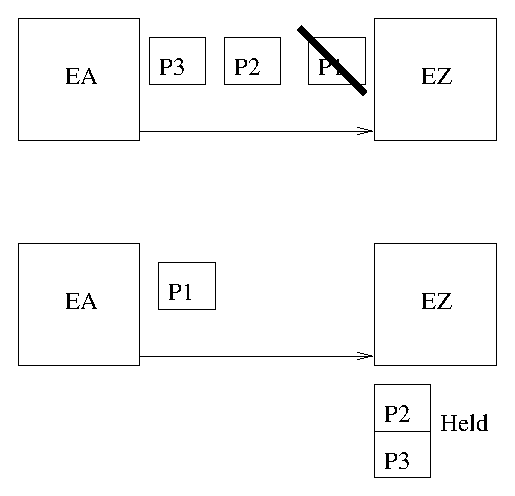
\includegraphics{lostpacket}
\caption{A lost packet}
\label{lost}
\end{figure}

Lets consider a TCP connection for a moment look at Fig~\ref{lost}. 
The sender, EA, sends Packets P1, P2 and P3. Note that to TCP the data
in each packet is dependent on what is on queue at the time TCP decided
to send the data, no message boundaries are implied by the packets. In this
transfer we have the unfortunate occurrence of a lost packet, P1 is lost. P2 and P3
arrive safely, but since the data is NOT in order they are held by the TCP stack
awaiting the retransmission of P1. This will usually happen within 1 second or so
depending on TCP's retransmission algorithms and timers.

Now what has happened is any data in P1 has caused a HOL condition in data
held within P2 and P3. In some cases, as we have stated, this may be very desirable.
But in many instances the information in P2 or P3 is not related to P1 (as we also
described above). This can cause delays in processing of information that may
be unacceptable to the application.

SCTP's streams were designed to deal with this very problem and provide a
method for applications to have finer grain control of what gets blocked by
the SCTP stack when such a packet loss occurs. When an application sends
data it can specify a stream number. There are up to 65,535 streams in an
SCTP association\footnote{The use of the term association is common and SCTP and represents a similar
concept to a TCP connection} (the exact number is negotiated at association startup).
When a message is sent in Stream N, a loss of data  that does not have
any Stream N data does not cause delays in delivery. In other words when data arrives
in a given stream (N) it is only held for reordering if other data is missing in that same stream.
So for example, lets assume that P1 contains a message for stream 11, P2 contains a message for stream 2 and 
P3 contains a message for stream 6. Only messages in stream 11 would be blocked by
the loss of P1 so both the payloads of P2 and P3 would not be held but delivered 
immediately upon arrival\footnote{This assumes of course no other losses have occurred}.
Streams allow an application to do selective ordering of messages. 

SCTP also provides another ordering constraint that mimics UDP i.e. none. An application
is allowed to send a message has ``unordered''. When an application sends in this
fashion then it is specifying that the data has \emph{no} order with respect to any other
data sent previously. An unordered message is placed into the delivery queue (often
times termed a socket buffer) immediately upon arrival. 

The combination of streams and unordered data provide powerful tools an application
can use to provide fine grain control over the delivery of data upon arrival at
the peer endpoint SCTP stack. Many applications in today's Internet can gain
improved performance in the face of network loss.

\subsection{Multihoming}
\label{multi}
The second of the two key features of SCTP is multihoming. A host that
is multihomed has more than one point of attachment to the network.
In a traditional TCP connection one set of IP address are chosen to 
send and receive packets over. The two IP addresses selected represent
1/2 of the four tuple identification of the connection (IP-A + Port-A, IP-Z + Port-Z).

In SCTP an association is composed of a two ``set's'' of IP addresses and two ports. This
means that if two hosts are multihomed all of their IP addresses can be involved
in sending and receiving data. In instances of lost packets SCTP will often select
one of the alternate addresses to send data to. This provides a form of network 
resilience in the face of loss and network outages. Consider Fig~\ref{mhomeloss}(a).
The network connection to EZ via IP3 has failed, and EA sends two packets P1 and P2 using
IP3 as the destination. Naturally the data will be lost, since there is an ``airgap''
between the network and the host. Later when EA's SCTP stack detects the loss (via timeout)
the retransmission would take the alternate path Fig~\ref{mhomeloss}(b). This gives
the application additional redundancy. When you combine this with the ability to fine tune
the retransmission timers (including the minimum and maximum values) an 
application can improve both its availability and how quickly it will recover from
errors..

An additional feature that many SCTP stacks offer is the ability to dynamically 
reconfigure the IP address set that makes up the association ~\cite{rfc5061}. This
provides the ability for an association to survive an address renumber or take
advantage of a hot-pluggable network interface without restarting the 
association. Again this unique feature provides yet again more support 
to an application attempting to minimize down time.

\begin{figure}]
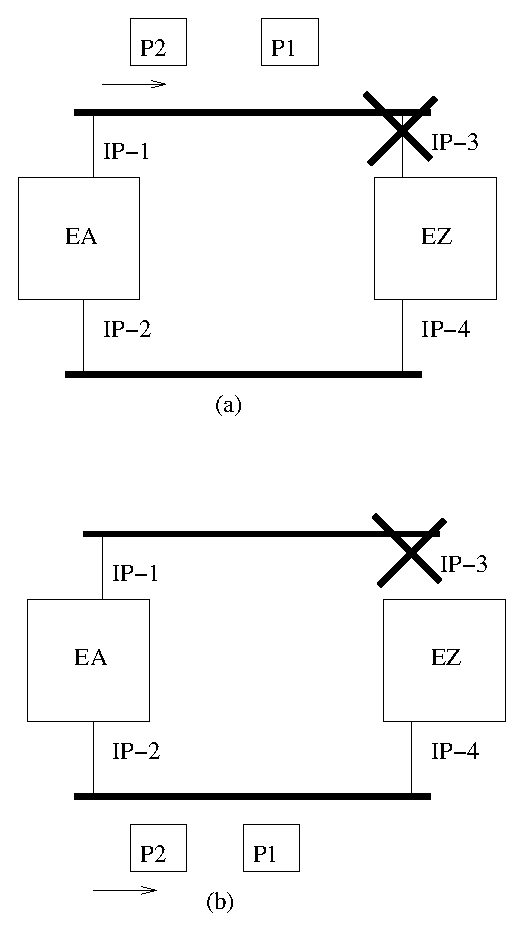
\includegraphics{multihome}
\caption{A multi-home loss}
\label{mhomeloss}
\end{figure}


\subsection{Partial Reliability}
\label{prsctp}
Partial Reliability, as the name implies, lets SCTP control the 
amount of reliability an application wants. Consider a video
game sending character position updates every 400 milliseconds.
If data is lost and not retransmitted within that time period (400ms) then
retransmitting the character position makes no sense when a new
updated one is already enqueue. With the addition of \cite{rfc3758} SCTP
gained the ability to specify how long a message is good for.  The initial
RFC allows the user to specify a ``time to live'' for a data packet. The 
sender makes a decision based on this ``time to live'' as to when to
skip over the data. 

The actual mechanism to skip over the data is separate from the
methodology used to determine when to skip over data. This means that
a sender can have many different ``profiles'' for skipping data and the
receiver does not need to have the same ``profile''.

Currently the authors are aware of three profiles commonly implemented:
\begin{itemize}
  \item Time based reliability
  \item Buffer based reliability
  \item Number of retransmissions
\end{itemize}
The time based profile follows RFC3758 in that the sender specifies
the number of milliseconds before the message should be skipped.  As
many retransmissions that are possible will be made in the time allowed.
So for example if the application sends the data with a 9,000 millisecond
reliability the message will be retransmitted several times\footnote{The exact
number of times is based on factors such as the minimum and maximum RTO} if loss occurs.

Another reliability profile is the so called buffer based. In this form the user specifies the maximum
number of bytes of data that is allowed to be on queue. If the size of the queue 
specified is reached, then the oldest data (marked in this manner) is looked to be
skipped so that the new data can be added to the queue of outgoing data.

The number of retransmissions profile allows an application to specify how many
times the data will be retransmitted. So, for example, if the application specified
zero times no retransmissions would be made\footnote{this is similar to UDP
except that this profiles assures that at least one transmission occurs whereas
UDP makes no such assurance}.

In all cases, no matter which profile is used, fully reliable and partially reliable
data may be mixed. In effect a single stream may have both reliable and
partially reliable data enqueued on it. This also as ramifications to the 
buffer based method in that if the entire association is filled with 
fully reliable data, then the new send itself will be the one subject
to ``skipping''.

\subsection{Message boundaries}
\label{mbound}
Message boundary preservation is a small incremental feature added to
SCTP but one that many developers will be happy to see. When you think of
an interaction between two applications rarely do they exchange a ``stream of bytes''.
Instead they send, receive and act upon messages. In a TCP connection each
message must be framed in some way. Any read of a buffer may return
parts of two separate messages. The application needs to provide application
layer code that parses the message based on the way the messages
were framed by the sender. 

With SCTP messages are never merged together upon reading. As long
as a large enough buffer is provided for reading, each read returns a 
single message. Each send is considered to be a message in itself\footnote{Note that
there are mechanisms to explicitly avoid this premise, but the default behavior is such
that every send is a message}. As a consequence the application does not need to
track by neither the sender or receiver where the message boundaries are.

Note that the message boundary preservation does have impact on how
messages are transmitted. SCTP is capable of bundling multiple messages
together and even splitting a large message over multiple Protocol Data Units (PDUs)
but how the bundling or splitting happens is often times driven by the size of the 
messages the user is sending and the Path Maximum Transport Unit (PMTU).


\subsection{Security}
\label{secure}

Security is a topic of  some importance since a transport protocol that is subject
to easy attack is not acceptable in todays often hostile Internet. SCTP has several
unique features that help strengthen its security to blind attacks and an optional
extension that takes that even further \cite{rfc4895}.

Every SCTP association starts with a four way handshake. This four
way handshake includes a signed cookie that the passive server side
sends to the active initiating client. The server holds no state and thus
is not subject to the SYN flooding attack. 

In the first two packets during the setup exchange a 32 bit random
value is supplied by both endpoints. All packets sent by one side must
have the verification tag (vtag) supplied during setup of the association in
order to be accepted by the receiving SCTP stack. This 32 bit vtag serves
as a 32 bit random nonce. This means that a blind attacker must generate
2 billion guess (on average) in order to say inject a ``ABORT'' chunk to tear
down the association. 

The authentication option RFC4895\cite{rfc4895} makes it so that any chunk can
be required to be signed in such a way so that the receiver can know
without doubt that the source was the sender. Even applications that
decide not to use shared keys can still gain some measure of security assuming
that the first two packets that setup an association are not intercepted by a
man in the middle.

Note that even though SCTP uses a four way handshake, this does not
cause delay in getting the first data messages to the receiver. In fact,
due to the way most TCP stack socket API's work, SCTP usually can get
the first data chunk to its peer one half of a round trip quicker than TCP.

\subsection{Other differences}
\label{miscdiff}

There are a few other differences worth noting in any comparison of
transports. One of the obvious differences is the checksum. In both
UDP and TCP a summation is used of all bits in the message. The summation
is done as a simple addition of all bytes in the message including a
pseudo-header. The pseudo-header is selected parts of the IP
header to help detect when a router mis-directs a packet. For SCTP
a Cyclic Redundancy Check is used (CRC32c). A CRC is much stronger
than a checksum and provides much better protection against
bit errors and packet damage done by routers and other network
devices. 

The Pseudo-header mentioned above is not needed in SCTP. The reason
is the vtag discussed earlier. The Pseudo-header, as noted, is used to
detect mis-routed packets in the checksum. For SCTP the 32 bit random
nonce provides this same protection without the need to embed a
hidden field in the packets checksum.

Another consequence of the use of a vtag is the absence of 
the timed-wait state in the protocol state machine. In TCP, for
some period of time after an endpoint shuts down, the TCP stack
prevents the port from being bound. This period of time is called
the ``timed-wait'' period and normally last for about
two minutes.  The purpose of this ``timed-wait'' is to allow
packets to drain from the network. In SCTP the vtag protects
us from this same situation as long as vtags themselves are
put into a ``timed-wait''.

SCTP also includes a required heartbeat mechanism. In contrast
TCP has an optional keep-alive mechanism which must be explicitly
enabled by the application. 

One other striking difference between TCP and SCTP is the absence
of the half closed state. In a TCP connection one side is allowed to
inform the peer that it will send no more data but will continue to accept
data from the peer. This state is known as half closed. SCTP does not
allow this behavior. If a user closes one side, then the connection will
shutdown.

\subsection{A word about optional features}
\label{options}
In the preceding sections we have mentioned several optional
features. So one may ask just which of them should I expect from
my implementation. It is the authors opinions that a complete 
SCTP implementation will include:
\begin{enumerate}
 \item  RFC4960 (basic SCTP)
 \item  RFC3758 (partial reliability)
 \item  RFC4895 (authentication)
 \item  RFC5061 (dynamic addresses)
\end{enumerate}

There are other drafts and extensions that are currently being
reviewed by the IETF but these will truly be optional in our
opinions. The ones listed above, however, though optional we
consider quite necessary for a full featured SCTP stack.

\section{Socket API overview}
So now that we have discussed some of the features and function of SCTP lets
talk about how you use this powerful new protocol. As with TCP and UDP, the socket
API is the most common method of accessing and using SCTP. Before diving deep into
the details of SCTP's socket API we will first get an overview of some of the
basic elements and choices that an application writer will have when using
SCTP.

\subsection{Models}
First and foremost when we go to use SCTP we have two choices. We can
use either the one-to-one model or the one-to-many model. So what exactly
are these two models, what do I gain from them and how do I access them?

The one-to-one model is a ``TCP'' compatibility model. Basically this model
works the same exact way that the standard TCP socket API model works.
A server will typically call \emph{socket()}, \emph{bind()}, and \emph{listen()}. Then after
the initial setup will sit in an loop calling \emph{accept()} to gain new connections.
Each new connection is a new socket descriptor on which the new
connection is available to send and data on. The application must track each individual socket
descriptor for each connection setup.  The client would do a call \emph{socket()}  followed by a call to \emph{connect()} to the
address of the server. 

The big advantage to this model is that a simple change to 
existing TCP code will make that code work with SCTP. To access this model a user
calls \emph{socket(int domain,  int type, int proto)}
with type set to SOCK\_STREAM and proto set to IPPROTO\_SCTP. 
Note that the domain argument is generally how you choose between IPv6 
and IPv4 (AF\_INET6 and AF\_INET).

The one-to-many model is unique to SCTP but has some characteristics of UDP.
It is designed as a peer-to-peer type model.  In this model both side generally
call \emph{socket()} followed by listen. Then when they wish to exchange information
with a peer they call \emph{sendto()} or \emph{recvfom()} (or any of the extended send or receive
calls (see section \ref{adv}). Note that the one single  socket will have multiple
associations underneath it. Only one socket descriptor is ever used for
in this model, calling \emph{accept()} will return an error. One of the big advantages to this model is the
ability to send data on the third leg of the four way handshake\footnote{Note that some 
implementations do allow this with the one-to-one model at the expense of
breaking TCP compatibility}. Another advantage is that an application does not
really need to track connection state. In order to be truly free of connection
state however the application is recommended to turn on the \emph{AUTO\_CLOSE} socket option
that will automatically close connections that are idle for long periods. 

Accessing the one to many model is done by calling the call specifying the type as
SOCK\_DGRAM and the proto as IPPROTO\_SCTP.

\subsection{Notifications}

While developing the socket API for SCTP it became quickly obvious
that the transport itself would often have things to say to the application 
(if the application is interested). The existing socket API had no method
for the transport to easily communicate events that were happening
on the transport. To deal with this the socket API for SCTP allows an
application to subscribe to ``notifications''. The subscription is
done via one of the SCTP \emph{setsockopt()} calls. Once a
notification is turned on, when the transport has an event to tell
the application it sends a message to the application up the normal
data path with the flags field set to \emph{MSG\_NOTIFICATION}. When a
user application does subscribe, it is in effect acknowledging to the SCTP stack
that it (the application) understands it must look at the flags field before interpreting
a message, since its possible its not a message from a peer but from the transport
itself.

There are current eight types of notifications. they are:
\begin{itemize}
 \item  Association events - the starting and closing of new associations
 \item  Address events - information about peer addresses, failures, additions, deletions, confirmations.
 \item  Send Failures - When a send fails, the data is returned with an error if you subscribe to this event.
 \item  Peer Error - If the peer sends an error message the stack would pass the TLV up the stack in this notification.
 \item  Shutdown events - Indications that a peer has closed or shutdown an association.
 \item  Partial delivery events - this notification will indicate issues that may occur in the partial delivery api.
 \item  Adaptation layer event - this notification holds a adaptation indication.
 \item  Authentication event - Various authentication events (such as new keys activated) would be signaled by this notification.
 \end{itemize}

Often applications will not be interested in a number of these notification. Two of the most
useful notifications for the one-to-many model is the Association and Shutdown events. Within
these events is an association identification often called assoc\_id. This identify's uniquely the
association that is in the one-to-many socket. It can actually be used with some of the extended
API calls to send to (instead of using a socket address).  Many of the socket options used with
SCTP will take the assoc\_id has an argument to identify changing or gathering settings on
a specific association instead of the whole socket descriptor.

We will discuss all of the notifications in detail in the next section.

\subsection{Extended calls}

All of the existing socket api calls will work with SCTP. There are
obviously limitations in either there utility or in there ease of use.
But they all will work seamlessly and can provide most to all of
the functions needed. However, there are a few corner cases
where the socket API just does not have adequate utility:

\begin{itemize}
 \item  For binding addresses, you can have one or all addresses.
 \item  For connecting to a peer you can connect to one and only one address.
 \item  For sending or receiving, getting access to the stream information is rather awkward.
\end{itemize}

To solve these problems there are extensions to the socket API to add
both ease of use and additional features. New ``system calls'' have been added
specifically for SCTP. Note that a system call may be no more than a utility library
routine that eases access to a specific feature. 

We will discuss each of the extended socket API calls as well as other features such
as notifications and socket options in \ref{adv}


\section{Socket API - details}
\label{adv}
So now that you have a general idea of the advantages of SCTP you are probably
wondering how you access these features. This section will try to highlight and provide
a rough overview of he way a user can best interact with SCTP.


\subsection{Notifications}

\subsection{Extended system calls}

\begin{itemize}
 \item  sctp\_connectx(int sd, struct sockaddr *, int addrcnt, sctp\_assoc\_t *)
 \item  sctp\_bindx(int sd, struct sockaddr *, int addrcnt, int type)
 \item  sctp\_recvmsg(int sd, void *msg, size\_t len, struct sockaddr *from, socklen\_t *fromlen, struct sctp\_sndrcvinfo *, int *flags)
 \item  sctp\_sendmsg(int s, void *msg, size\_t len, struct sockaddr *to, socklen\_t tolen, uint32\_t ppid, uint32\_t flags, uint16\_t stream, uint32\_t timetolive, uint32\_t context)
 \item  sctp\_sendmsgx(int s, void *msg, size\_t len, struct sockaddr *to, int addrcnt, socklen\_t tolen, uint32\_t ppid, uint32\_t flags, uint16\_t stream, uint32\_t timetolive, uint32\_t context)
 \item  sctp\_send(int sd, void *msg, size\_t len, struct sctp\_sndrcvinfo *, int flags)
 \item  sctp\_sendx(int sd, void *msg, size\_t len, struct sockaddr *addrs, int addrcnt, struct sctp\_sndrcvinfo *, int flags)
\end{itemize}

\subsection{Socket Options}

\begin{table}
\begin{tabular}{|l|r|l|}
\hline
Option & R-W & Description\\
\hline \hline
SCTP\_RTOINFO & rw & RTO min/max\\
\hline
SCTP\_ASSOCINFO & rw & Association parameters\\
\hline
SCTP\_INITMSG & rw & Setup options\\
\hline
SCTP\_NODELAY & rw & Nagle algorithm\\
\hline
SCTP\_AUTOCLOSE & rw & Automatic closing\\
\hline
SCTP\_SET\_PEER\_PRIMARY\_ADDR & rw & Remote primary\\
\hline
SCTP\_PRIMARY\_ADDR & rw & Local primary\\
\hline
SCTP\_ADAPTATION\_LAYER & rw & AI indication\\
\hline
SCTP\_DISABLE\_FRAGMENTS & rw & Fragmentation\\
\hline
SCTP\_PEER\_ADDR\_PARAM & rw & Misc parameters\\
\hline
SCTP\_DEFAULT\_SEND\_PARAMS & rw & Default sendrcvinfo\\
\hline
SCTP\_EVENTS & rw & Notifications\\
\hline
SCTP\_I\_WANT\_MAPPED\_V4\_ADDR & rw & Mapped v4 addresses\\
\hline
SCTP\_MAXSEG & rw & Fragmentation point\\
\hline
SCTP\_DELAYED\_SACK & rw & Delayed sack\\
\hline
SCTP\_FRAGMENT\_INTERLEAVE & rw & Receive interleave\\
\hline
SCTP\_PARTIAL\_DELIVERY\_POINT & rw & receive PD point\\
\hline
SCTP\_AUTH\_CHUNK & w & Add Auth Chunk\\
\hline
SCTP\_AUTH\_KEY & w & Add auth key\\
\hline
SCTP\_HMAC\_IDENT & rw & hmac algo\\
\hline
SCTP\_AUTH\_ACTIVE\_KEY & rw & Active key\\
\hline
SCTP\_AUTH\_DELETE\_KEY & w & Delete key\\
\hline
SCTP\_USE\_EXT\_RCVINFO & rw & Extended sndrcvinfo\\
\hline
SCTP\_AUTO\_ASCONF & rw & Automatic IP add/del\\
\hline
SCTP\_MAXBURST & rw & Microburst control\\
\hline
SCTP\_CONTEXT & rw & Default context\\
\hline
SCTP\_EXPLICTI\_EOR & rw & Explict EOR\\
\hline
SCTP\_STATUS & r & Assoc status\\
\hline
SCTP\_GET\_PEER\_ADDR\_INFO & r & Info on dest\\
\hline
SCTP\_PEER\_AUTH\_CHUNKS & r & peer requires auth\\
\hline
SCTP\_LOCAL\_AUTH\_CHUNKS & r & local requires auth\\
\hline
SCTP\_GET\_ASSOC\_NUMBER & r & Num of assocs\\
\hline
SCTP\_GET\_ASSOC\_ID\_LIST & r & Assoc ids\\
\hline
\end{tabular}
\caption{SCTP Socket Options\label{sockopt}}
\end{table}

\begin{table}
\begin{tabular}{|l|r|l|}
\hline
Option & R-W & Description\\
\hline \hline
SCTP\_RESET\_STREAMS & w & Stream reset\\
\hline
SCTP\_SET\_DEBUG\_LEVEL & rw & Debug output\\
\hline
SCTP\_CMT\_ON\_OFF & rw & CMT on/off\\
\hline
SCTP\_CMT\_USE\_DAC & rw & DAC with CMT\\
\hline
SCTP\_PLUGGABLE\_CC & rw & Set CC\\
\hline
SCTP\_GET\_SNDBUF\_USE & r &  send space\\
\hline
SCTP\_GET\_NONCE\_VALUES & r & Vtag pair\\
\hline
SCTP\_SET\_DYNAMIC\_PRIMARY & w & Global primary\\
\hline
SCTP\_GET\_PACKET\_LOG & r & Packet log \\
\hline
SCTP\_VRF\_ID & rw & Defaut vrf\\
\hline
SCTP\_ADD\_VRF\_ID & w & Add a VRF\\
\hline
SCTP\_GET\_VRF\_IDS & r & Get VRF IDs\\
\hline
SCTP\_GET\_ASOC\_VRF & r & Asoc VRF ID\\
\hline
SCTP\_DEL\_VRF\_ID & w & Del VRF ID\\
\hline
\end{tabular}
\caption{SCTP FreeBSD Specific Socket Options\label{sockopt}}
\end{table}


\subsection{Some Examples}


\section{Conclusion}

\section*{Acknowledgment}


The authors would like to thank...


\begin{thebibliography}{11}
\bibitem{rfc4960} R.~Stewart,
  ``Stream Control Transmission Protocol'',
  \textit{RFC~4960},
  September~2007
.\bibitem{rfc793}  J~Postel,
  ``Transmission Control Protocol'',
  \textit{RFC~793},
  September~1981
.\bibitem{rfc768}  J~Postel,
  ``User Datagram Protocol'',
  \textit{RFC~768},
  August~1980
.\bibitem{rfc5061}  R~Stewart et.al.,
  ``Stream Control Transmission Protocol Dynamic Address Reconfiguration'',
  \textit{RFC~5061},
  September~2007
.\bibitem{rfc3758}  M~Tuexen et.al.,
 ``Stream Control Transmission Protocol Partial Reliability Extension'',
  \textit{RFC~3758},
  May~2004
.\bibitem{rfc4895}  R~Stewart et.al.,
  ``Authenticated Chunks for the Stream Control Transmission Protocol'',
  \textit{RFC~4895},
  August~2007


\end{thebibliography}




% that's all folks
\end{document}


